\documentclass[tikz,border=6pt]{standalone}
\usepackage{tikz}
\usetikzlibrary{arrows.meta,positioning,calc}
\usepackage{pgfplots}

%% fonts
\usepackage{dsfont}
\usepackage[T1]{fontenc}
\usepackage{lmodern}
\usepackage{amsmath}
\usepackage{caption}

\begin{document}

\begin{tikzpicture}[scale=1.0]
  % overall box
  \draw[thick] (0,0) rectangle (8,8);

  % thresholds (choose positions you like)
  \def\tone{3.0}  % t1 on X1
  \def\tthree{5.2}% t3 on X1
  \def\ttwo{3.2}  % t2 on X2
  \def\tfour{6.0} % t4 on X2

  % vertical splits
  \draw[thick] (\tone,0) -- (\tone,8);
  \draw[thick] (\tthree,0) -- (\tthree,8);

  % horizontal splits
  \draw[thick] (0,\ttwo) -- (\tone,\ttwo);              % left block
  \draw[thick] (\tthree,\tfour) -- (8,\tfour);          % right block

  % labels for regions
  \node at (1.5,1.6) {$R_1$};
  \node at (1.5,5.5) {$R_2$};
  \node at (4.1,4.0) {$R_3$};
  \node at (6.5,2.6) {$R_4$};
  \node at (6.5,7.0) {$R_5$};

  % axis labels and ticks
  \node[below] at (4,-0.8) {$X_1$};
  \node[left, rotate=90] at (-0.8,4) {$X_2$};

  \draw (\tone,0) -- ++(0,-0.15) node[below] {$t_{1}$};
  \draw (\tthree,0) -- ++(0,-0.15) node[below] {$t_{3}$};

  \draw (0,\ttwo) -- ++(-0.15,0) node[left] {$t_{2}$};
  \draw (8,\tfour) -- ++(0.15,0) node[right] {$t_{4}$};
\end{tikzpicture}

\begin{tikzpicture}[
  grow=down,
  level 1/.style={sibling distance=40mm, level distance=23mm},
  level 2/.style={sibling distance=30mm, level distance=23mm},
  level 3/.style={sibling distance=30mm, level distance=23mm},
  edge from parent/.style={draw,-,thick},
  every node/.style = {font=\large},
  scale=1.0
  ]

\node {$X_1 \leq t_1$}
  child {node {$X_2 \leq t_2$}
    child {node {$R_1$}}
    child {node {$R_2$}}
  }
  child {node {$X_1 \leq t_3$}
    child {node {$R_3$}}
    child {node {$X_2 \leq t_4$}
      child {node {$R_4$}}
      child {node {$R_5$}}
    }
  };

\end{tikzpicture}

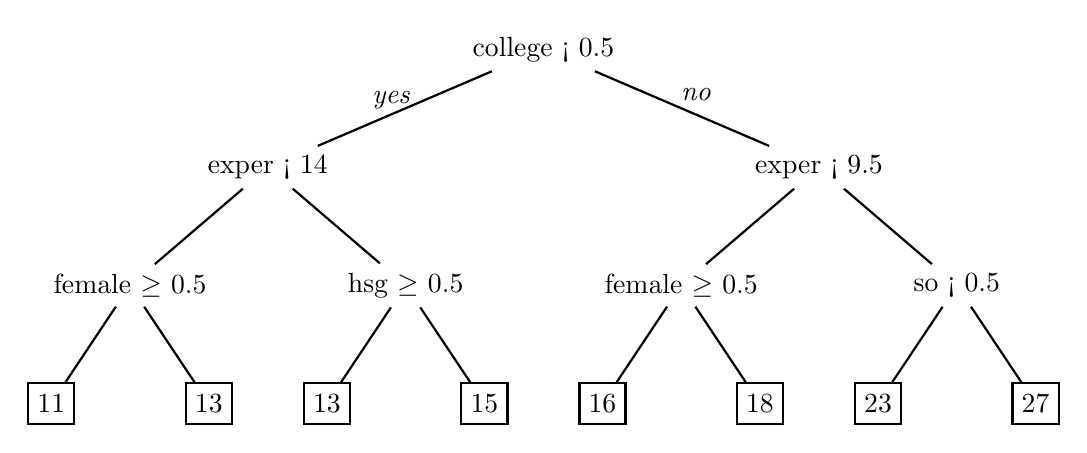
\begin{tikzpicture}[
  grow=down,
  level 1/.style={sibling distance=70mm, level distance=15mm},
  level 2/.style={sibling distance=35mm, level distance=15mm},
  level 3/.style={sibling distance=20mm, level distance=15mm},
  edge from parent/.style={draw, -, thick},
  every node/.style = {align=center, font=\normalsize},
  leaf/.style = {draw, minimum width=1em, minimum height=1.5em}
]

\node (root) {college < 0.5}
  child {node {exper < 14}
    child {node {female $\geq$ 0.5}
      child {node [leaf] {11}}
      child {node [leaf] {13}}
    }
    child {node {hsg $\geq$ 0.5}
      child {node [leaf] {13}}
      child {node [leaf] {15}}
    }
  }
  child {node {exper < 9.5}
    child {node {female $\geq$ 0.5}
      child {node [leaf] {16}}
      child {node [leaf] {18}}
    }
    child {node {so < 0.5}
      child {node [leaf] {23}}
      child {node [leaf] {27}}
    }
  };

% Add "yes" and "no" near the first branch
\node[font=\itshape, above left=10pt and -8em of root-1] {yes};
\node[font=\itshape, above right=13pt and -8em of root-2] {no};

\end{tikzpicture}


\end{document}